%% ------------------------------------------------------------------------- %%
\chapter{Introdução}
\label{cap:introducao}


A predição da resistência compressiva do cimento (CCS) é reconhecida como de
extrema importância para a indústria da construção civil, pois essa
capacidade é um dos fatores para avaliar a qualidade do cimento
\citep{cementml}. O CCS após 28 dias da produção do cimento (RC28) é escolhido
 como um parâmetro regulatório em normas de construção. Dado que os custos
 anuais de manutenção de estruturas são da ordem de bilhões de dólares, métodos
 estatísticos para a predição dessa quantidade ainda na fase de fabricação ganha ainda mais importância para o
 funcionamento mais eficiente da indústria. Nota-se também que essa  
 indústria representa grande parte das emissões de $CO_2$ na atmosfera \citep{cementroadmap}.

Esse trabalho é uma colaboração entre a empresa Intercement, o Laboratório de
Lógica, Inteligência Artificial e Métodos Formais do IME-USP e o Departamento de
Construção Civil da POLI-USP. Foram apresentados
10 anos de dados de diversas etapas da produção de cimento do complexo de
Cajati, uma das plantas da empresa. Esse trabalho estuda a possibilidade do uso
de modelos computacionais e estatísticos modernos em dados produzidos diariamente nas fábricas,
para a tomada de decisões na operação da fábrica.


\section {Motivação}



Trabalhos recentes aplicam técnicas estatísticas em amostras de cimento num
contexto laboratorial \citep{cementlin,nncement}.
Nosso objetivo é estender a metodologia para
levar essas análises da operação da fábrica, com dados colhidos na operação diária que já
possam entregar resultados imediatos para a ação dos operadores.

O trabalho \citep{dynstat} propõe uma regressão linear cujos parâmetros são recalculados
sempre que um novo valor RC28 é amostrado pelo laboratório. Nossa contribuição é
o tratamento completo dos dados providenciados na operação da fábrica como
\textbf{séries temporais} i.e. dados indexados por anotações de tempo.

Por muitas décadas o estado da arte desse tipo de análise temporal centrou-se
nos processos ARIMA, com a metodologia Box-Jenkins \citep{arima}.
Esses modelos têm uma excelente capacidade estatística e interpretabilidade.
Mas essa família de modelos possui suas limitações:
ela falha em modelar relações não-lineares nos dados \citep{forecasting} e 
muitos processos reais tendem a ser não-lineares por natureza.
Esses modelos também têm dificuldade de incorporar variáveis exógenas à série temporal nas predições \citep{ubertime}.


A modelagem de série temporais tem se beneficiado pelo desenvolvimento de novos
métodos de Aprendizado de Máquina (ML), e mais recentemente de Aprendizado Profundo (DL).
Modelos de DL diferem de abordagens estatísticas clássicas por serem orientados
a dados \citep{dlbook}.
Esses modelos não necessitam de \textit{feature engineering}, e também não
assumem muito sobre a distribuição geradora dos dados, como por exemplo a
família ARIMA, que requisita do engenheiro de dados a especificação da
sazonalidade e estacionariedade dos dados \citep{arima}.
Redes Neurais são capazes de aprender sozinhas diversas características dos dados sem necessidade de intervenção. 
Alguns trabalhos uniram a flexibilidade de redes neurais com a robustez de
métodos ARIMA \citep{DIAZROBLES20088331,KHASHEI2010479},
criando soluções melhores que qualquer um desses modelos sozinho. Porém, uma das
arquiteturas de DL mais presentes atualmente em análise de séries temporais
são as Redes Neurais Recorrentes. Esses modelos já foram usados com
melhores resultados do que métodos clássicos para prever séries temporais de
demanda de energia elétrica e de carros em um aplicativo de corridas popular
\citep{energylstm,ubertime}.


Nossa metodologia deve ser capaz de prever o sensível nível de imprecisão e
incerteza que ocorre no processo industrial,
refletindo assim as condições reais observadas na fábrica. A estatística bayesiana oferece técnicas
mais robustas para a modelagem de incerteza \citep{bayesml}. E num contexto em
que possuímos muitos dados, técnicas de DL também podem ser aplicadas com um desenvolvimento bayesiano para a propagação de erro e cálculo de incertezas \citep{ubertime,Gal2016Uncertainty}. 



%% ------------------------------------------------------------------------- %%
\section{Produção de Cimento}
\label{sec:producao}

Nessa seção a produção de cimento será brevemente descrita, usando como base a Figura~\ref{fig:cimento}:  

\begin{figure}[H]
\centering
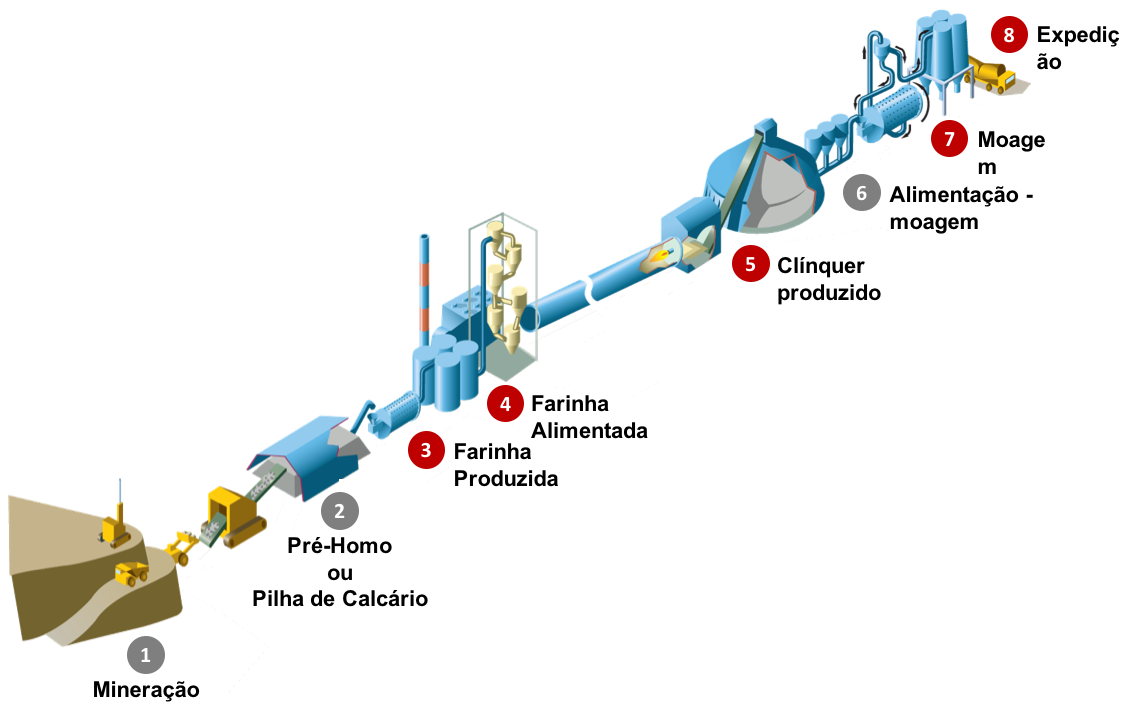
\includegraphics[width=0.9\columnwidth]{cimento.png}
\caption{Representação das Diversas Etapas da produção de Cimento \citep{cementroadmap}}
\label{fig:cimento}
\end{figure}


As etapas de produção serão explicadas por número como indicado na imagem: \\

\begin{itemize}

\item[1] Depósitos ricos em carbonato de cálcio são minerados para extração desse químico. Normalmente a planta é próxima da mina.
\item[2] O material extraído é triturado em pedaços de até 10cm de diâmetro. Diferentes materiais são misturados ao resultado da tritura, de modo a manter a composição química desejada. 
\item[3] A farinha crua é pré-aquecida para que depois no forno as reações químicas aconteçam mais rápido. 
\item[4] O carbonato de cálcio é transformado em CaO por meio de reações químicas.  
\item[5] O material é introduzido ao forno, atingindo temperaturas de até $1450^\circ$C, transformando a farinha em clínquer. O clínquer é resfriado após a saída do forno. 
\item[6] O clínquer então é misturado com outros componentes que formam o cimento.
\item[7] A mistura é então moída.
\item[8] O material é empacotado, estocado e eventualmente expedido para entrega.

\end{itemize}

Os dados de interesse nesse projeto são medições de diversos parâmetros em meio ao processo de fabricação do cimento. Eles são divididos em diversas planilhas para diferentes etapas da produção de cimento, são elas, em ordem no processo:

\begin{itemize}
        \item Cimento Cru
        \item Farinha
        \item Clinquér
        \item Produção de Cimento
        \item Expedição de Cimento (Saco e Granel)
\end{itemize}

Dado que não existe uma maneira trivial de combinar dados de partes diferentes do processo (é muito difícil acompanhar o mesmo lote de cimento/matéria prima em partes diferentes do processo), as análises serão feitas em cima dos dados de Expedição de Cimento.

\subsection{Índice de Resistência de Cimento Portland}
\label{sec:rc}
A propriedade que iremos tentar prever usando nossos modelos será a resistência
compressiva do cimento. A resistência de uma amostra de cimento é ensaiada em
intervalos determinados de dias após a sua confecção. Essas informações são
anotadas nos dados com os nomes de $RCn$, com $n$ sendo a idade da amostra em
dias. Esses índices possuem a unidade de kPa, i.e. quilopascal.

%% ------------------------------------------------------------------------- %%
\section{Objetivos}
\label{sec:objetivo}

Gostaríamos no desenvolvimento desse trabalho de obter resultados com a
aplicação de técnicas de DL recentes para um domínio inédito: Usando a
natureza temporal dos dados para predizer os valores de RC28 com dados diários
produzidos no chão de fábrica. Dessa maneira
estaremos abrindo portas para uma presença de aprendizado estatístico no processo de
engenharia da produção de cimento. De modo que esses modelos possam ser usados para tomadas de decisão no chão de fábrica.


%% ------------------------------------------------------------------------- %%
\section{Organização do Trabalho}
\label{sec:organizacao_trabalho}

No Capítulo~\ref{cap:conceitos}, apresentamos os conceitos de Aprendizado de
Máquina, estatística frequentista e bayesiana, estimadores, métricas de acurária
e uma breve explicação de cada modelo usado. É feita também uma introdução à inferência
bayesiana, e uma possível aproximação numérica dessa técnica. No
Capítulo~\ref{cap:estudodados} são apresentadas características gerais dos
dados e testes estatísticos sobre propriedades desses. No
Capítulo~\ref{cap:resultados} enumerados as transformações necessárias para usar
os dados em modelos sequenciais e resultados de predições e métricas de
acurária de todos os modelos. No Capítulo~\ref{cap:conclusoes} são apresentadas
direções para pesquisa futura e palavras finais. 



%%% Local Variables:
%%% mode: latex
%%% TeX-master: "../quali"
%%% End: